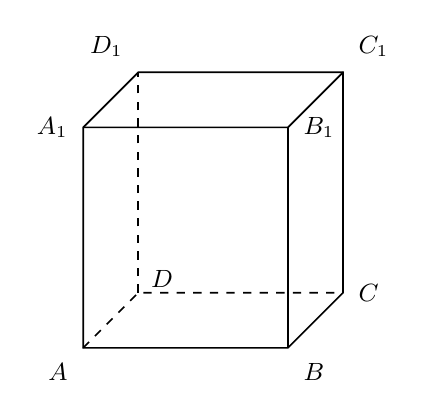
\begin{tikzpicture}[line width=.6pt,font=\small]
\coordinate (A) at (0,0);
\coordinate (B) at (2.6,0);
\coordinate (C) at (3.3,0.7);
\coordinate (D) at (0.7,0.7);
\coordinate (A1) at (0,2.8);
\coordinate (B1) at (2.6,2.8);
\coordinate (C1) at (3.3,3.5);
\coordinate (D1) at (0.7,3.5);
\draw[dashed] (A) -- (D) -- (C);
\draw[dashed] (D) -- (D1);
\draw (A) -- (B) -- (C) -- (C1) -- (D1) -- (A1) -- cycle;

\draw (B) -- (B1);
\draw (A1) -- (B1) -- (C1);

\node[below left,xshift=-2pt,yshift=-2pt] at (A) {$A$};
\node[below right,xshift=2pt,yshift=-2pt] at (B) {$B$};
\node[right,xshift=2pt] at (C) {$C$};
\node[right,xshift=1pt,yshift=5pt] at (D) {$D$};
\node[left,xshift=-2pt] at (A1) {$A_{1}$};
\node[right,xshift=2pt] at (B1) {$B_{1}$};
\node[above right,xshift=2pt,yshift=2pt] at (C1) {$C_{1}$};
\node[above left,xshift=-2pt,yshift=2pt] at (D1) {$D_{1}$};
\end{tikzpicture}
